\section{The \ToolName System: Architecture and Training Pipeline}
\label{sec:architecture}

\begin{figure}
    \centering
        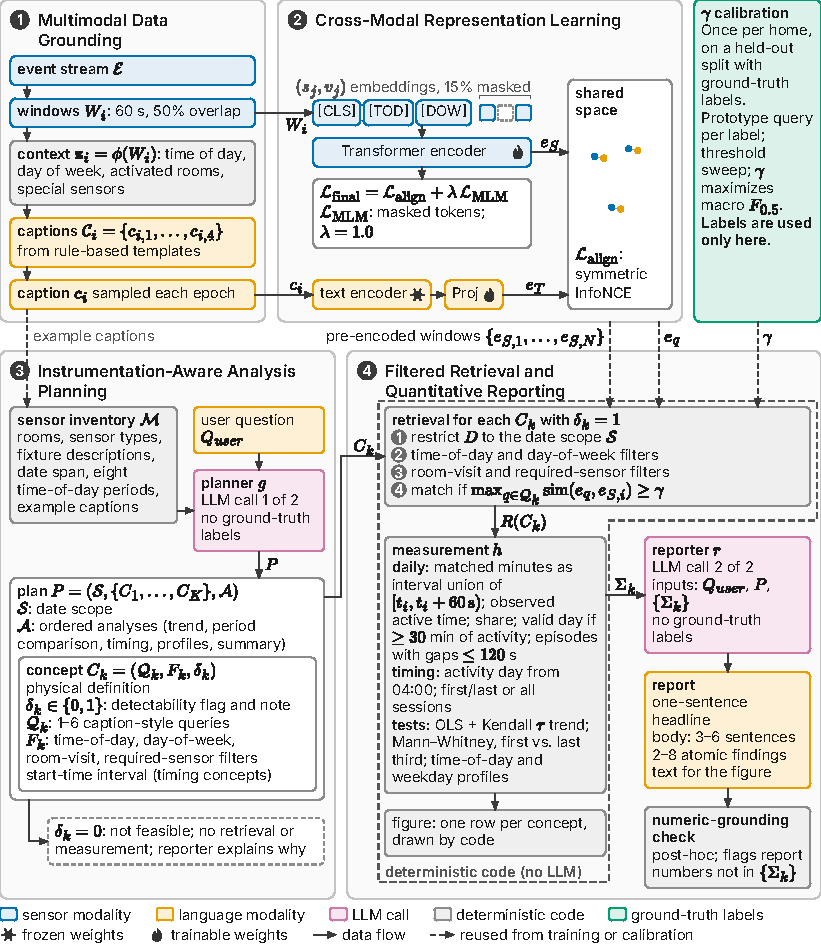
\includegraphics[width=\linewidth]{figures/model_architecture.pdf}
    \caption{
        Training Architecture Details. === FULL CAPTION TO BE ADDED ===
    }
    \vspace*{-1em}
    \label{fig:model_architecture}
\end{figure}

To address the limitations of the label-centric paradigm in smart home research, we introduce \ToolName, a framework for the multimodal encoding, semantic retrieval, and quantitative analysis of ambient sensor data. \ToolName aligns raw sensor sequences with natural language descriptions in a shared latent space. This alignment allows users to query household data using arbitrary natural language, effectively turning the smart home into a searchable behavioral database. An analysis layer built on top of this retrieval capability translates free-text questions about a resident into structured, sensor-grounded measurements and a written report. An overview of the system architecture, spanning from data ingestion to report generation, is provided in Figure~\ref{fig:model_architecture}.

The \ToolName framework is organized around four stages that enable the transition from raw sensor data to searchable and quantifiable behavioral insights. This architecture establishes a continuous pipeline that grounds physical signals in a semantic embedding space and then grounds language-level questions in that same space.

\begin{itemize}
    \item \textbf{Multimodal Data Grounding}:
    The framework begins by partitioning raw sensor event streams into temporal sequences. These sequences are paired with template-based captions that describe underlying movement patterns in natural language, creating the semantic foundation required for cross-modal alignment.

    \item \textbf{Cross-Modal Representation Learning}:
    To capture the latent structure of resident behavior, a deep temporal encoder is trained to identify co-occurrence patterns and transition dynamics within the sensor data. By employing a contrastive learning objective against a frozen language model, the system aligns these learned sensor signatures with high-level semantic knowledge, resulting in a unified representation space where sensor sequences are directly addressable via natural language.

    \item \textbf{Instrumentation-Aware Analysis Planning:} A planning step translates an abstract user question into a structured analysis plan that is conditioned on the physical sensor inventory of the home. The plan decomposes the question into observable behavioral concepts, each with caption-style retrieval queries, hard filters, a date scope, and a set of analyses to run; concepts that the home's sensors cannot observe are marked as such and excluded.

    \item \textbf{Filtered Retrieval and Quantitative Reporting:} The retrieval queries of each concept are projected into the shared embedding space and matched against the household's longitudinal database, subject to the plan's filters. Deterministic code converts the matched windows into daily measurements, timing statistics, and significance tests. A reporting step then produces a short written answer and a set of atomic findings constrained to the computed numbers.
\end{itemize}

The following sections provide a comprehensive discussion of the data processing pipeline, the training procedure, the analysis layer, and the specific implementation details of \ToolName.


\subsection{Problem Formulation}
\label{sec:problem_formulation}

\paragraph{Human Activity Retrieval.}
Let $D$ be a time-series dataset of smart home sensor readings partitioned into a set of temporal windows $D = \{W_1, W_2, \dots, W_n\}$. Each window $W_i$ represents a sequence of sensor events $\{s_1, s_2, \dots, s_l\}$. Traditional Human Activity Recognition (HAR) seeks to learn a mapping $f: W \to Y$, where $Y$ is a finite set of $k$ predefined activity labels.
The Human Activity Retrieval (HART) task removes the closed-set requirement of $Y$. Instead, it aims to retrieve a subset of relevant sensor windows $W^q \subseteq D$ that semantically correspond to a natural language query $q$. This is achieved by learning a joint embedding space into which both sensor sequences and linguistic queries are projected. The HART function is defined as:

\begin{equation}
f_{\text{HART}}(q, D) = \{ W_i \in D \mid \text{sim}(e_{q}, e_{W_i}) \geq \gamma \}
\label{eq:hart}
\end{equation}

where $e_q$ and $e_{W_i}$ are the vector representations of the query and sensor window, respectively, $\text{sim}(\cdot,\cdot)$ is cosine similarity, and $\gamma$ is a similarity threshold. This formulation enables a flexible, open-vocabulary search that captures the unique behavioral patterns and sensing capabilities of an individual smart home.

\paragraph{Question answering over retrieved activity.}
A caregiver's question is typically not a retrieval query. It may refer to several distinct behaviors, to a time of day, to a change over time, or to a behavior that the home's sensors cannot observe at all. The analysis layer of \ToolName therefore mediates between a free-text user question $Q_{user}$ and the HART function. Let $\mathcal{M}$ denote the sensor inventory of the household (Section~\ref{sec:query_processing}). A planner $g$ maps the question and the inventory to an analysis plan:

\begin{equation}
g(Q_{user}, \mathcal{M}) \to P = \big(\mathcal{S},\, \{C_1, C_2, \dots, C_K\},\, \mathcal{A}\big)
\end{equation}

where $\mathcal{S}$ is a date scope, $\mathcal{A}$ is an ordered set of analyses to run, and each concept $C_k = (\mathcal{Q}_k, F_k, \delta_k)$ consists of a set of retrieval queries $\mathcal{Q}_k = \{q_{k,1}, \dots, q_{k,m_k}\}$, a set of hard filters $F_k$, and a detectability flag $\delta_k \in \{0, 1\}$. For each detectable concept, retrieval generalizes Equation~\ref{eq:hart} to a set of queries and the plan's filters:

\begin{equation}
R(C_k) = \Big\{ W_i \in D_{\mathcal{S}} \cap F_k \;\Big|\; \max_{q \in \mathcal{Q}_k} \text{sim}(e_q, e_{W_i}) \geq \gamma \Big\}
\label{eq:concept_retrieval}
\end{equation}

where $D_{\mathcal{S}}$ is the subset of $D$ within the date scope and $W_i \in F_k$ denotes that the window satisfies every filter in $F_k$. A deterministic measurement function $h$ maps $R(C_k)$ to a set of statistics $\Sigma_k$ (Section~\ref{sec:measurement}), and a reporter $r(Q_{user}, P, \{\Sigma_k\})$ produces the final written answer (Section~\ref{sec:reporting}). Concepts with $\delta_k = 0$ are not retrieved or measured; the reporter is required to state that the corresponding part of the question is not answerable in this home and why.


\subsection{Data Stream Processing and Automated Captioning}
\label{sec:data_processing}

The raw sensor readings from a smart home environment are represented as a continuous stream of events $\mathcal{E} = \{ (s_k, v_k) \}_{k=1}^K$, where $s_k$ denotes the unique sensor identifier (e.g., a motion sensor in the kitchen or a cabinet contact sensor) and $v_k$ is the discrete event value (e.g., OPEN, CLOSED, ON, OFF). Following previous work on smart home data processing \cite{civitarese2025_adl_llm}, we partition this stream into the set of temporal windows $D = \{W_1, W_2, \dots, W_n\}$. Each window $W_i$ covers a fixed duration of 60 seconds; consecutive windows overlap by 50\%, and each contains a variable-length sequence of $L_i$ events:

\begin{equation}
W_i = \{ (s_j, v_j) \}_{j=1}^{L_i}
\end{equation}

For each window $W_i$, we generate a corresponding set of natural language descriptions to facilitate the learning of the shared embedding space. We define a metadata extraction function $\phi(W_i) \rightarrow \mathbf{z}_i$, which aggregates context from the sensor events and the household's specific instrumentation. The context vector $\mathbf{z}_i$ includes the time of day, day of the week, the set of activated rooms, and triggers from specialized sensors, such as pressure mats or refrigerator contact sensors.

Using this metadata, we employ a rule-based captioning procedure to generate a set of four linguistically diverse variants $\mathcal{C}_i = \{c_{i,1}, c_{i,2}, c_{i,3}, c_{i,4}\}$. These variants capture the same underlying behavior through different syntactical structures and levels of abstraction. For example, for a segment in the kitchen during a Tuesday afternoon, the generator might produce:

\begin{itemize}
    \item $c_{i,1}$: The resident is in the kitchen using the refrigerator on a Tuesday afternoon.
    \item $c_{i,2}$: Activity detected in the kitchen involving the fridge during the day on Tuesday.
\end{itemize}

During the training phase, to encourage the model to learn robust and invariant semantic representations, we sample a single caption $c_i$ uniformly at random from the set $\mathcal{C}_i$ in each epoch. While we also explored the use of large language models to augment these descriptions with more semantically diverse narratives, empirical evaluations showed that the rule-based templates were sufficient for high-quality alignment (see Appendix, Section~\ref{sec:captioning_strategies}). Consequently, we utilize the template-based approach as our primary captioning strategy to ensure computational efficiency and scalability across large longitudinal datasets.


\subsection{Sensor Sequence Encoder}
\label{sec:sensor_encoder}

To encode discrete and asynchronous sensor events into a dense representation, following \cite{karpekov2025discover, transformers_for_smarthome2025, hiremath2022bootstrapping} we employ a Transformer-based architecture that captures the relationships between events in a sequence. This encoder transforms raw event sequences into behavioral signatures that can be mapped into the shared semantic space.

Each partitioned window $W_i$ consists of a variable-length sequence of sensor events $\{(s_j, v_j)\}_{j=1}^{L_i}$. To process these events, we first map each unique sensor identifier $s_j$ and discrete event value $v_j$ pair to a corresponding learnable embedding. This transformation yields a sensor embedding matrix $S \in \mathbb{R}^{L \times d}$, where $d$ is the model's embedding dimension. To handle variable sequence lengths within a training batch, we pad sequences to a maximum length $L_{max}$ and utilize an attention mask during the encoding process.

To provide the model with the temporal context, we prepend two specialized context tokens to each sequence:
\begin{enumerate}
    \item Time of Day: \texttt{[TOD]}: A categorical token representing one of eight distinct periods (e.g., early morning, late morning, early afternoon, etc.).
    \item Day of Week: \texttt{[DOW]}: A categorical token representing the specific day the activity occurred.
\end{enumerate}
These tokens are treated as non-maskable identifiers that provide a global temporal anchor for the sequence. They are initialized as learnable embeddings and are optimized solely through the cross-modal alignment loss discussed in ~\cref{sec:contrastive_alignment}, ensuring they capture the semantic relevance of timing to specific behaviors.

The final input sequence is constructed by prepending a learnable \texttt{[CLS]} token followed by the \texttt{[TOD]} and \texttt{[DOW]} tokens to the sensor embedding matrix $S$. This results in a final input representation:
\begin{equation}
S' \in \mathbb{R}^{(L+3) \times d}
\end{equation}
The input $S'$ is passed through a series of Transformer blocks. To obtain a fixed-size vector representation $e_S \in \mathbb{R}^{d}$ for the entire sequence, we extract the final hidden state of the \texttt{[CLS]} token:
\begin{equation}
e_S = \text{Encoder}(S')_{\texttt{CLS}}
\end{equation}
This $e_S$ vector represents the full sequence and its temporal context, serving as the sensor-modality anchor for the subsequent cross-modal alignment.


\subsection{Text Encoder and Projection}
\label{sec:text_encoder_details}

For each sensor window $W_i$, the corresponding sampled caption $c_i$ is processed using a frozen, pretrained text encoder. Following our benchmarking of various language models (see Section~\ref{sec:encoder_sensitivity}), we utilize a transformer-based text backbone trained on a diverse corpus of language pairs, allowing it to capture robust semantic relationships between common physical activities and their natural language descriptions. We keep the weights of this text encoder frozen throughout the alignment process to prevent the model from overfitting to the relatively low linguistic diversity of our template-based captions and to ensure it retains the general-purpose semantic knowledge required for open-vocabulary retrieval.

To map the fixed-size output of the text encoder into the shared latent space used for alignment, we employ a learnable projection head that transforms the encoder space into the aligned representation space. Formally, the final text embedding $e_T \in \mathbb{R}^d$ is calculated as:
\begin{equation}
e_T = \text{Proj}(\text{Encoder}(c_i))
\end{equation}
where $c_i$ is the input caption. This embedding $e_T$ serves as the linguistic target that the sensor sequence encoder must learn to approximate during the training phase.


\subsection{Alignment Training}
\label{sec:contrastive_alignment}

The objective of the HART training stage is to optimize the sensor encoder so that its representations are both internally coherent and semantically aligned with the natural language space. To achieve this, we employ a multi-task learning objective that combines cross-modal contrastive alignment with a unimodal masked language modeling task.

To align the sensor and text modalities, we utilize the InfoNCE loss \cite{oord2019representation}, which encourages the model to maximize the similarity between matched sensor-caption pairs while minimizing the similarity for all other mismatched pairs within a training batch $\mathcal{B}$. Let $e_S^i$ and $e_T^i$ be the sensor and text embeddings, respectively, for the $i^{\text{th}}$ example in the batch. The sensor-to-text alignment loss is defined as:

\begin{equation}
    \mathcal{L}_{S\rightarrow T} = -\frac{1}{|\mathcal{B}|} \sum_{i \in \mathcal{B}} \log \frac{\exp(\text{sim}(e_S^i, e_T^i) / \tau)}{\sum_{j \in \mathcal{B}} \exp(\text{sim}(e_S^i, e_T^j) / \tau)}
    \label{eq:loss_st}
\end{equation}

where $\text{sim}(\cdot, \cdot)$ denotes cosine similarity and $\tau$ is a learnable temperature parameter. We define a symmetric text-to-sensor loss $\mathcal{L}_{T\rightarrow S}$ in an identical fashion, resulting in the total alignment loss:

\begin{equation}
    \mathcal{L}_{\text{align}} = \mathcal{L}_{S\rightarrow T} + \mathcal{L}_{T\rightarrow S}
\end{equation}

While the contrastive loss establishes a global semantic mapping, it does not explicitly force the model to learn the fine-grained dependencies between individual sensor events. To address this, we introduce a unimodal Masked Language Modeling (MLM) objective for the sensor encoder. During training, we randomly mask 15\% of the input sensor tokens. The encoder is then tasked with predicting the identity of the masked sensor-value pairs based on the surrounding sequential context.

We apply a standard cross-entropy loss for this reconstruction task, denoted as $\mathcal{L}_{\text{MLM}}$. This objective serves as a regularizer and encourages the model to reason about the co-occurrence patterns inherent to a specific household.
The final training objective is the weighted sum of the two losses:

\begin{equation}
    \mathcal{L}_{\text{final}} = \mathcal{L}_{\text{align}} + \lambda \mathcal{L}_{\text{MLM}}
    \label{eq:loss_final}
\end{equation}

where we set $\lambda = 1.0$ to give equal importance to global semantic alignment and local sequence modeling. This dual-objective approach ensures that the resulting embeddings are semantically rich enough for open-vocabulary retrieval while remaining grounded in the physical dynamics of the actual sensor readings.


\subsection{Instrumentation-Aware Analysis Planning}
\label{sec:query_processing}

To bridge the gap between abstract user intent and the specific physical capabilities of a household, the analysis layer of \ToolName begins with a planning step that serves as the function $g(Q_{user}, \mathcal{M})$ of Section~\ref{sec:problem_formulation}. The planner is implemented as a single call to a Large Language Model (LLM) with a fixed schema for its output (Section~\ref{sec:implementation}). It receives the user question verbatim together with a description of the home's sensing, and it returns an analysis plan. Ground-truth activity labels are never provided to the planner.

\paragraph{Sensor inventory.}
The inventory $\mathcal{M}$ is constructed from the household metadata. It lists, for every sensor, its room identifier, sensor type, and a short description of the fixture it monitors (e.g., a contact sensor on a refrigerator door), together with the date span of the recorded data and the eight time-of-day periods used by the \texttt{[TOD]} token. The inventory also includes a small number of example captions drawn from the embedding model's training data, so that the planner's queries are phrased in the vocabulary the sensor encoder was aligned to. The planner is instructed that only the listed rooms and fixtures exist in the home.

\paragraph{Plan structure.}
The plan $P$ contains (i) an interpretation of the question and explicit caveats, such as the use of a proxy behavior, the presence of multiple residents, or a short recording span; (ii) one concept $C_k$ per distinct behavior the question refers to; (iii) a date scope $\mathcal{S}$; and (iv) an ordered list of analyses $\mathcal{A}$, with the primary analysis first, drawn from a fixed set: trend, period comparison, timing, time-of-day profile, day-of-week profile, and overall summary. Relative temporal expressions in the question (e.g., ``recently'') are resolved against the end of the recorded data rather than the date of the call; an unspecified bound defaults to the start or end of the available series.

\paragraph{Concept decomposition.}
Each concept carries a one-sentence physical definition that a human rater can verify on a floor-plan replay of the sensor data. A scheduled behavior that recurs at separate times of day (e.g., breakfast, lunch, and dinner; morning and evening medication; wake-up and bedtime) is split into one concept per occurrence, each with its own time-of-day filter and with the time of day written into every query. Because the sensor encoder is conditioned on time of day (Section~\ref{sec:sensor_encoder}), this phrasing biases retrieval toward the intended period before any hard filter is applied.

\paragraph{Detectability.}
The planner is instructed that ambient motion and door contact sensors observe presence, dwell, movement between rooms, and door use, but not posture, objects, appliances, lock state, or hand actions. For each concept, it sets the detectability flag $\delta_k$ and writes a detectability note. If a behavior can only be approximated by a proxy, the note states the proxy. If the behavior cannot be observed with the listed sensors, $\delta_k = 0$ and the query list is empty; the concept is then excluded from retrieval, measurement, and sampling, and the reporter must state that this part of the question is not feasible in this home and why. Every concept must be grounded in the inventory: a door, room, or fixture with no listed sensor is not feasible, and the planner is instructed not to substitute another sensor in its place.

\paragraph{Retrieval queries.}
Each detectable concept has between one and six retrieval queries $\mathcal{Q}_k$. Queries are caption-style sentences that describe observable behavior rather than an activity-label name, contain no sensor identifiers, and refer to a single place or movement pattern each, since a disjunction within one sentence retrieves poorly in the shared embedding space.

\paragraph{Hard filters.}
The filter set $F_k$ is applied after embedding-based retrieval and only when a filter is part of the concept's definition. Four filters are available: a time-of-day filter over the eight periods; a day-of-week filter; a room filter, under which a window must \emph{visit} at least one listed room (a visit rather than a dominant-room criterion, because, for example, a bathroom trip within a 60-second window is usually dominated by bedroom events); and a required-sensor filter, under which at least one listed sensor must fire ON or OPEN within the window, used for door-related concepts. For concepts analyzed by timing (Section~\ref{sec:measurement}), the plan additionally specifies the clock-time interval in which an occurrence may start (breakfast $[5, 11)$, lunch $[11, 15)$, dinner $[16, 21)$, wake-up $[4, 12)$, and bedtime $[19, 3)$ hours), chosen so that the intervals of different occurrences of the same behavior do not overlap.


\subsection{Filtered Semantic Retrieval}
\label{sec:retrieval_strategy}

Each detectable concept is executed against the household's longitudinal database $D$, whose 60-second windows have been pre-encoded by the sensor encoder into $\{e_{S,1}, e_{S,2}, \dots, e_{S,N}\}$. The procedure implements Equation~\ref{eq:concept_retrieval} in four steps:

\begin{enumerate}
    \item Restrict $D$ to the date scope $\mathcal{S}$ of the plan.
    \item Apply the time-of-day and day-of-week filters.
    \item Apply the room-visit and required-sensor filters. The number of windows matched before this step is stored alongside the final count, so that embedding-only retrieval can be compared with filtered retrieval.
    \item Encode each query $q \in \mathcal{Q}_k$ with the frozen text encoder and projection head of Section~\ref{sec:text_encoder_details}. The score of a window is the maximum cosine similarity over the concept's queries, and a window is a match if its score is at least $\gamma$.
\end{enumerate}

The threshold $\gamma$ is calibrated once per home on a held-out split with ground-truth labels. For each activity label we form a prototype query from its template caption, retrieve with Equation~\ref{eq:hart} at a range of thresholds, and select the cosine cutoff that maximizes macro-averaged $F_{0.5}$ across labels. We use $F_{0.5}$ rather than $F_1$ to weight precision above recall at the operating point; the empirical motivation for this choice is given in Section~\ref{sec:retrieval_threshold}. Labels are used only for this calibration and do not enter the analysis layer. Experiments that use a fixed number of nearest neighbors instead of a threshold are identified as such where they are reported.


\subsection{Behavioral Measurement}
\label{sec:measurement}

All measurements are computed by deterministic code from the matched windows $R(C_k)$ and the windows in scope.

\paragraph{Daily quantities.}
Because consecutive windows overlap, matched windows are not counted as separate minutes. The \emph{matched minutes} of a day are the Lebesgue measure of the union of the intervals $[t_i, t_i + 60\,\text{s})$ over all matched windows $W_i$ starting on that day, where $t_i$ is the window start time. The same union, taken over every window in the date scope that passes the time-of-day and day-of-week filters, is the day's \emph{observed active time}. The \emph{share} of a day is matched minutes divided by observed active time. Room-visit and required-sensor filters are applied to the numerator only, so share is the fraction of the resident's activity during the concept's time filters that resembles the behavior. A separate validity rule guards against sparse days: a day's total in-scope sensor activity, computed as the same interval union over all windows in the date scope without any time-of-day or weekday restriction, must reach 30 minutes. Days below this threshold are marked invalid and excluded from the daily means, the trend, the period comparison, the timing analysis, and the figure. Matched windows are grouped into \emph{episodes} by merging windows separated by at most 120 seconds. The headline quantities of a concept are matched minutes per day, episodes per day, median episode length, and share of active time. A matched minute is one minute of sensor activity whose window resembles the described behavior; it is not the duration of the behavior itself. Share is a secondary quantity, since it changes when the resident's other activity changes even if the behavior's own minutes do not.

\paragraph{Timing.}
Amount statistics cannot answer when a behavior occurs. The timing analysis operates on matched sessions only and does not use the observed-active-time denominator; it retains the same valid days as the daily series. It assigns episodes to \emph{activity days} that begin at 04:00, so that an event at 01:00 belongs to the preceding evening. Two modes are available. In the \emph{first}/\emph{last} mode (e.g., wake-up or bedtime), one clock time per activity day is extracted and summarized by its median, interquartile range, the percentage of days on which the event was observed, a Kendall trend of clock time in minutes per week, and a Mann--Whitney comparison of the last third of days against the first third, or against the periods named in the plan. In the \emph{all} mode (e.g., meals or medication), every session is retained and summarized by its typical hours and the consistency with which they recur. Sessions for timing may use a wider merging gap and a minimum session length than episodes (for meals, 30 and 5 minutes respectively); momentary events keep the 120-second episode gap. Sessions are formed from matches at any time of day and are retained if they start inside the concept's start-time interval, so that a period boundary does not clip the start of a session. We observed that time-of-day words in a query pull retrieval mass toward the minutes immediately after a period boundary. If more than 30\% of days place the event within 10 minutes after such a boundary, the statistics are flagged and the reporter is instructed to state that the true start may be earlier and not to treat that clock time or its tight spread as the resident's schedule.

\paragraph{Statistical tests.}
A \emph{trend} is estimated on valid days by ordinary least squares of the daily value on days elapsed since the first day, together with Kendall's $\tau$ on the same pairs. For both share and minutes per day the output reports the slope per week, $\tau$ and its $p$-value, the fitted values on the first and last day, and the relative change of the fitted line; a trend is flagged as significant when the Kendall $p$-value of the share series is below 0.05. A \emph{period comparison} tests the first third of valid days against the last third, by default, with a two-sided Mann--Whitney $U$ test on daily share. \emph{Profiles} report matched minutes, observed minutes, and share per time-of-day period and per weekday. Profiles are computed independently of the daily series: for each period or weekday, observed minutes are the interval union over all windows in the date scope that fall in that period or weekday, without the concept's filters, and matched minutes are the union over the concept's matched windows in the same period or weekday. The validity rule is not applied to profiles.


\subsection{Report Generation}
\label{sec:reporting}

The reporter is the second and final LLM call. It receives the user question, the plan, and the statistics $\{\Sigma_k\}$ with internal bookkeeping fields removed. It produces a one-sentence headline, a body of three to six sentences, a list of findings, and the text that accompanies a figure. Ground-truth activity labels are not provided.

\paragraph{Numeric grounding.}
The reporter may only use numbers that appear in the statistics. A post-hoc check extracts every number in the report and flags any that does not match a value in the statistics payload up to rounding; integers from 0 to 10 are exempt from this check.

\paragraph{Wording rules.}
Trend language is tied to the tests: a significant trend is described as ``increased'' or ``decreased''; otherwise the report states ``no clear trend'' or describes a slight change that is not statistically reliable. The same rule applies to clock-time shifts (``shifted'' versus ``no clear shift'').

\paragraph{Findings.}
The report includes between two and eight atomic findings. Each finding refers to exactly one concept, is of exactly one kind (\emph{level}, \emph{change}, \emph{timing}, \emph{comparison}, or \emph{pattern}), and is a single statement of roughly 20 words or fewer. A finding states one amount or one change, never both. No finding may refer to a concept that was not analyzed, and no finding may consist solely of a restatement of a limitation. This structure allows each finding to be rated independently by a human reviewer.

\paragraph{Figure.}
Each report is accompanied by a figure with one row per analyzed concept. For amount concepts, the row shows a scatter of the daily share of active time, a 7-day moving mean, the fitted share trend line, a small table of share by time-of-day period, and a floor plan of the home with bubbles sized by the number of sensor activations within matched windows. Timing concepts show a scatter of clock times per activity day in place of the share scatter.


\subsection{Implementation Details}
\label{sec:implementation}

The planner and reporter are the only components of the analysis layer that generate language; retrieval, filtering, measurement, statistical tests, and figures are deterministic. Both LLM calls use Gemini 3.1 Pro (\texttt{gemini-3.1-pro-preview}) with structured JSON output conforming to the plan and report schemas, thinking level \texttt{high}, and temperature 1.0. Each response is cached under a key formed by hashing the model identifier, the system prompt, the user prompt, the output schema, the thinking level, and the temperature, so that a complete run can be replayed offline from the cached responses. Window embeddings for the longitudinal index are computed with the retrieval model of Section~\ref{sec:contrastive_alignment} at a maximum sequence length of 256 events.